% Foliensatz: "AFu-Kurs nach DJ4UF" von DK0TU, Amateurfunkgruppe der TU Berlin
% Lizenz: CC BY-NC-SA 3.0 de (http://creativecommons.org/licenses/by-nc-sa/3.0/de/)
% Autoren:
% Martin Deutschmann <martin.deutschmann@campus.tu-berlin.de>
% Korrekturen:
% Lars Weiler <dc4lw@darc.de>

\documentclass[aspectratio=169]{beamer}

\usepackage[ngerman]{babel} % deutsche Worttrennung etc.
\usepackage[utf8]{inputenc} % UTF8 Text

\usepackage[super, comma, numbers, square, sort]{natbib}

\usepackage{hyperref}       % Hyperref Package für bessere Referenzen (todo)
\hypersetup{
	colorlinks=false,       %   false: boxed links; true: colored links
    %linkcolor=white,       %   color of internal links (change box color with linkbordercolor)
    citecolor=red,          %   color of links to bibliography
    filecolor=white,        %   color of file links
    urlcolor=blue           %   color of external links
}

\usepackage{multirow}
\usepackage{wasysym}  % Math Symbols like \permil
%\usepackage{colortbl}
%\usepackage{subscript}
%\usepackage{caption}
%\usepackage{setspace}
%\usepackage{xcolor}        % benutze CodeListe

% Footnote
%\usepackage{hanging}
%
%\setbeamertemplate{footnote}{%
%  \hangpara{2em}{1}%
%  \makebox[2em][l]{\insertfootnotemark}\footnotesize\insertfootnotetext\par%
%}


%\usepackage{pgf}
%\usepackage{tikz}
%\usetikzlibrary{arrows,automata}
%\usetikzlibrary{positioning}
%
%\tikzset{
%    state/.style={
%           rectangle,
%           rounded corners,
%           draw=black, very thick,
%           minimum height=2em,
%           minimum width=2pt,
%           inner sep=2pt,
%           text centered,
%           },
%}

%\usepackage{listings}
%\lstset{basicstyle=\small, numberstyle=\tiny, extendedchars=true, numbers=left, numbersep=5pt}
%\lstset{showtabs=false, showspaces=false, showstringspaces=false}
%%\lstset{backgroundcolor=\color{white!75!lightgray}, , frame=single}
%%\lstset{backgroundcolor=\color{white}}
%%\lstset{backgroundcolor=none}
%\lstset{keywordstyle=\color{blue!50!gray},  identifierstyle=\color{black}}
%\lstset{commentstyle=\color{green!50!gray}, stringstyle=\color{red!50!gray}}
%\lstset{language=C, fontadjust=true, tabsize=2, breaklines=true}
%\lstset{backgroundcolor=\color{white!75!lightgray}, caption=\lstname, frame=single}
%\lstset{emphstyle=\color{black}\fbox}
%
%% Keine "Listing:"-Caption
%\captionsetup{labelformat=empty,labelsep=none}
%
%% für mathematische Umgebungen
%\usepackage{amsmath,amsfonts,amssymb}
%
%\lstdefinestyle{Bash}{
%language=Bash,
%frame=single,
%rulecolor=\color{black},
%backgroundcolor=\color{gray!50},
%keywordstyle=\color{black},
%identifierstyle=,
%commentstyle=\color{black},
%stringstyle=\color{magenta!65!white},
%showstringspaces=false,
%basicstyle=\footnotesize\ttfamily\color{black},
%numbers=none,
%breaklines=true,
%captionpos=b
%}

%\usepackage{listings}
%
%\lstdefinestyle{basic}{
%    captionpos=t,%
%    basicstyle=\footnotesize\ttfamily,%
%    numberstyle=\tiny,%
%    numbers=left,%
%    stepnumber=1,%
%    frame=single,%
%    showspaces=false,%
%    showstringspaces=false,%
%    showtabs=false,%
%    %
%    keywordstyle=\color{blue},%
%    identifierstyle=,%
%    commentstyle=\color{gray},%
%    stringstyle=\color{magenta}%
%}



% fließende Boxen haben keinen Abstand
%\fboxsep0mm

% inkludiere Creative Commons Helper
%%%%%%%%%%%%%%%%%%%%%%%%%%%%%%%%%%%%%%%%%%%%%%%%%%%%%%%%%%%%%%%%
%% ccBeamer 0.1, 2007-07-02                                   %%
%% Written by Sebastian Pipping <webmaster@hartwork.org>      %%
%% ---------------------------------------------------------- %%
%% Licensed under Creative Commons Attribution-ShareAlike 3.0 %%
%% http://creativecommons.org/licenses/by-sa/3.0/             %%
%%%%%%%%%%%%%%%%%%%%%%%%%%%%%%%%%%%%%%%%%%%%%%%%%%%%%%%%%%%%%%%%


%% Images
\newcommand{\CcImageBy}[1]{%
	
\includegraphics[scale=#1]{texdata/creative_commons/cc_by_30.pdf}%
}
\newcommand{\CcImageCc}[1]{%
	
\includegraphics[scale=#1]{texdata/creative_commons/cc_cc_30.pdf}%
}
\newcommand{\CcImageDevNations}[1]{%
	
\includegraphics[scale=#1]{texdata/creative_commons/cc_dev_nations_30.pdf}%
}
\newcommand{\CcImageNc}[1]{%
	
\includegraphics[scale=#1]{texdata/creative_commons/cc_nc_30.pdf}%
}
\newcommand{\CcImageNd}[1]{%
	
\includegraphics[scale=#1]{texdata/creative_commons/cc_nd_30.pdf}%
}
\newcommand{\CcImagePd}[1]{%
	
\includegraphics[scale=#1]{texdata/creative_commons/cc_pd_30.pdf}%
}
\newcommand{\CcImageSa}[1]{%
	
\includegraphics[scale=#1]{texdata/creative_commons/cc_sa_30.pdf}%
}
\newcommand{\CcImageSampling}[1]{%
	
\includegraphics[scale=#1]{texdata/creative_commons/cc_sampling_30.pdf}%
}
\newcommand{\CcImageSamplingPlus}[1]{%
	
\includegraphics[scale=#1]{texdata/creative_commons/cc_sampling_plus_30.pdf}%
}


%% Groups
\newcommand{\CcGroupBy}[2]{% zoom, gap
	\CcImageCc{#1}\hspace*{#2}\CcImageBy{#1}%
}
\newcommand{\CcGroupByNc}[2]{% zoom, gap
	\CcImageCc{#1}\hspace*{#2}\CcImageBy{#1}\hspace*{#2}\CcImageNc{#1}%
}
\newcommand{\CcGroupByNcNd}[2]{% zoom, gap
	\CcImageCc{#1}\hspace*{#2}\CcImageBy{#1}\hspace*{#2}\CcImageNc{#1}\hspace*{#2}\CcImageNd{#1}%
}
\newcommand{\CcGroupByNcSa}[2]{% zoom, gap
	\CcImageCc{#1}\hspace*{#2}\CcImageBy{#1}\hspace*{#2}\CcImageNc{#1}\hspace*{#2}\CcImageSa{#1}%
}
\newcommand{\CcGroupByNd}[2]{% zoom, gap
	\CcImageCc{#1}\hspace*{#2}\CcImageBy{#1}\hspace*{#2}\CcImageNd{#1}%
}
\newcommand{\CcGroupBySa}[2]{% zoom, gap
	\CcImageCc{#1}\hspace*{#2}\CcImageBy{#1}\hspace*{#2}\CcImageSa{#1}%
}
\newcommand{\CcGroupDevNations}[2]{% zoom, gap
	\CcImageCc{#1}\hspace*{#2}\CcImageDevNations{#1}%
}
\newcommand{\CcGroupNcSampling}[2]{% zoom, gap
	\CcImageCc{#1}\hspace*{#2}\CcImageNc{#1}\hspace*{#2}\CcImageSampling{#1}%
}
\newcommand{\CcGroupPd}[1]{% zoom
	\CcImagePd{#1}%
}
\newcommand{\CcGroupSampling}[1]{% zoom
	\CcImageSampling{#1}%
}
\newcommand{\CcGroupSamplingPlus}[1]{% zoom
	\CcImageSamplingPlus{#1}%
}


%% Text
\newcommand{\CcLongnameBy}{Attribution}
\newcommand{\CcLongnameByNc}{Attribution-NonCommercial}
\newcommand{\CcLongnameByNcNd}{Attribution-NoDerivs}
\newcommand{\CcLongnameByNcSa}{Attribution-NonCommercial-ShareAlike}
\newcommand{\CcLongnameByNd}{Attribution-NoDerivs}
\newcommand{\CcLongnameBySa}{Attribution-ShareAlike}

\newcommand{\CcNote}[1]{% longname
	This work is licensed under the \textit{Creative Commons #1 3.0 License}.%
}


% generelles Thema auswählen
\usetheme{Goettingen} %Berlin spart ohne Sidebar allerdings angenehm Platz
% AnnArbor | Antibes | Bergen | Berkeley | Berlin | Boadilla | boxes | CambridgeUS | Copenhagen | Darmstadt | default | Dresden | Frankfurt | Goettingen | Hannover | Ilmenau | JuanLesPins | Luebeck | Madrid | Malmoe | Marburg | Montpellier | PaloAlto | Pittsburgh | Rochester | Singapore | Szeged | Warsaw

% Farben wählen
\usecolortheme{beetle}
% beaver | beetle | crane | default | dolphin | dove | fly | lily | orchid | rose | seagull | seahorse | sidebartab | structure | whale | wolverine

% Setze alle Farben auf Grau und Weiß
%\definecolor{craneorange}{RGB}{64,64,64}
%\definecolor{craneblue}{RGB}{255,255,255}

% Schriftart wählen
\usefonttheme{default}
% default | professionalfonts | serif | structurebold | structureitalicserif | structuresmallcapsserif

% Innere Themen(Kopf-, Fuß-, Sidebar usw)
%\useinnertheme{default}
\useinnertheme{circles}
% default | inmargin | rectangles | rounded | circles

% Äußere Themen (Anordnung der inneren, grenzen der Folien etc.)
\useoutertheme{infolines}
% default | infolines | miniframes | shadow | sidebar | smoothbars | smoothtree | split | tree

% Deaktiviere Navigations-Symbole ({} -> leer)
\setbeamertemplate{navigation symbols}{}
%\setbeamertemplate{navigation symbols}{\large \ifnum \insertframenumber <10 0\fi\insertframenumber/\inserttotalframenumber\vspace*{0.2ex}}

% Zeige ein Hintergrundbild
\setbeamertemplate{background canvas}{
        \hspace*{-2.0cm}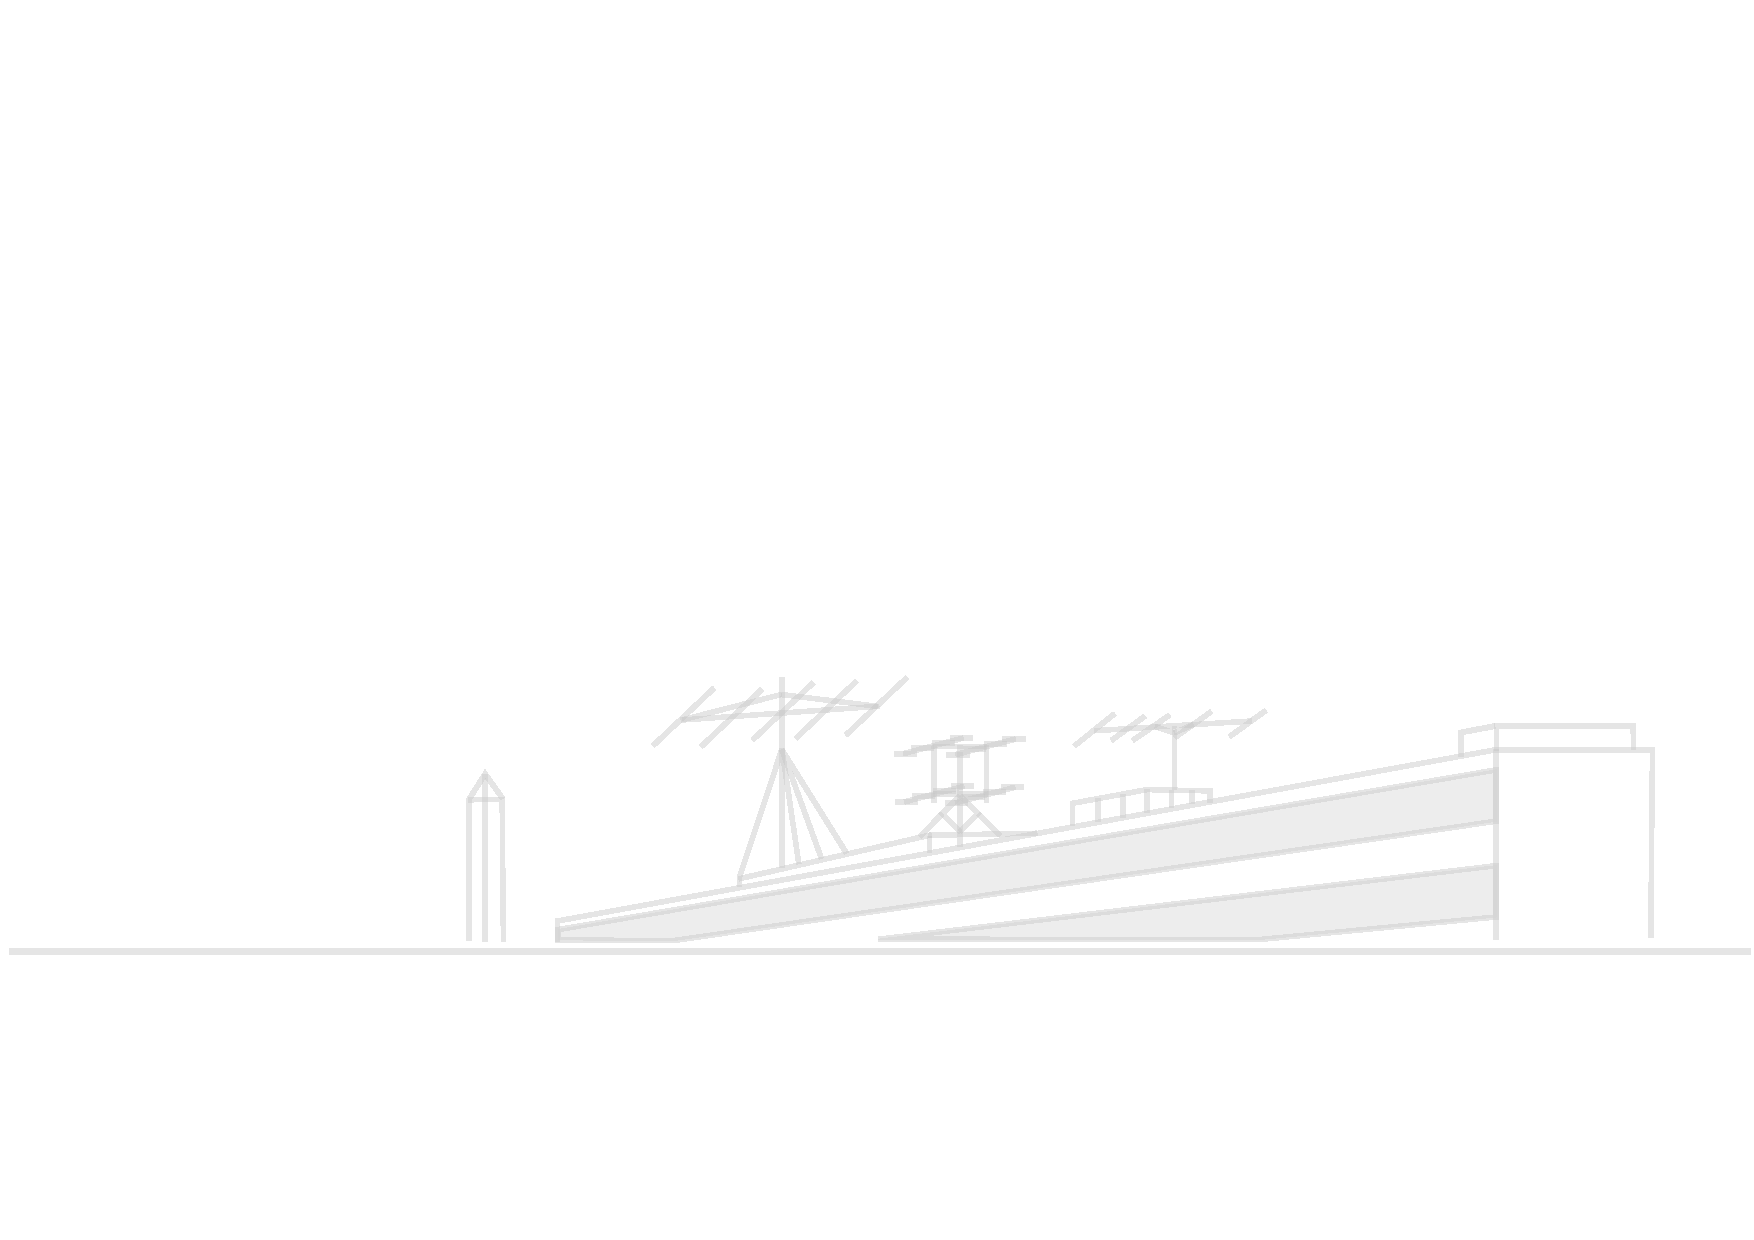
\includegraphics[width=17.8cm]{texdata/dk0tu_rooftop_background.pdf}
}

% Foliennummer einfügen
\setbeamertemplate{footline}[frame number]
%\setbeamertemplate{footline}{}

% Ändere das Zeichen vor jedem item
%\setbeamertemplate{itemize item}{\color{craneorange}$\blacktriangleright$}
%\setbeamertemplate{itemize subitem}{\color{craneorange}$\triangleright$}
%\setbeamertemplate{itemize subsubitem}{\color{craneorange}$\blacktriangleright$}

% Ändert die Blöcke 
\setbeamertemplate{blocks}[rounded][shadow=true]
% default | rounded [shadow=true|false]

%
% Eigene Kommandos
%

% Hack to get natbib and beamer working together. "The beamer user guide suggests
% that only the manual bibliography entry approach is supported"
% on some system it works out of the box, sometimes you need the hack :-(
% so check it --dl7bst
\ifdefined\newblock
    \relax
\else
    \newcommand{\newblock}{}
\fi

% \includedia command to generate png out of a dia file
% NEEDS installed dia and pdflatex option --shell-escape
\newcommand{\includedia}[1]{
    \immediate\write18{/usr/bin/dia #1.dia -e #1_diatmp.png -t png}
}

% RICHIG GROSSER FONT!
\newfont{\bigfont}{cmr10 at 144pt}
\newfont{\smallfont}{cmr10 at 8pt}

% Römische Ziffern
\makeatletter
\newcommand{\rmnum}[1]{\romannumeral #1}
\newcommand{\Rmnum}[1]{\expandafter\@slowromancap\romannumeral #1@}
\makeatother

% Schwarze Überschrift
%\setbeamercolor{frametitle}{fg=black}
%\setbeamercolor{title}{fg=black}

% Item- und Box-Farben
\definecolor{deepBlue}{HTML}{000066}
\setbeamercolor{itemize item}{fg=deepBlue}
\setbeamercolor{itemize subitem}{fg=deepBlue}
\setbeamercolor{description item}{fg=deepBlue}
\setbeamercolor{block title}{fg=deepBlue!100, bg=blue!15}
\setbeamercolor{block body}{fg=black, bg=blue!5}
\setbeamercolor{block title alerted}{fg=deepBlue, bg=red!75}
\setbeamercolor{block body alerted}{fg=black, bg=red!15}
\setbeamercolor*{block title example}{fg=blue!50, bg=blue!10}
\setbeamercolor*{block body example}{fg= blue, bg=blue!5}

%\setbeamercolor{section in head/foot}{parent=palette primary}
%\setbeamercolor{subsection in head/foot}{parent=palette secondary}
%\setbeamercolor{sidebar}{fg=darkblue,bg=yellow!90!orange}
%\setbeamercolor{title in sidebar}{fg=darkblue}
%\setbeamercolor{author in sidebar}{fg=darkblue}
%\setbeamercolor{section in sidebar}{fg=darkblue!10!black}
%\setbeamercolor{subsection in sidebar}{fg=darkblue!50!black}

% Titlepage Infos
\title{AFu-Kurs nach DJ4UF}
\author[DKØTU]{DKØTU\\ \footnotesize{Amateurfunkgruppe der TU Berlin}}
\institute[DKØTU]{\url{http://www.dk0tu.de} }

% PDF-Eigenschaften
\subject{DK0TU-Amateurfunkkurs nach DJ4UF}
\keywords{Amateurfunk Kurs HAM Radio Course CC-BY-NC-SA OpenSource TU Berlin DK0TU}

\subtitle{Technik Klasse E 18 \& Betriebstechnik/Vorschriften 14: \\
  EMV, EMVG, EMVU, Sicherheit \& Störungen  \\[2em]}
\date{Stand 19.12.2016}
 \begin{document}

\begin{frame}
    \titlepage
    \vfill
    \begin{center}
        \ccbyncsaeu\\
        {\tiny This work is licensed under the \em{Creative Commons Attribution-NonCommercial-ShareAlike 3.0 License}.}\\[0.5ex]
         \tiny Amateurfunkgruppe der Technische Universität Berlin (AfuTUB), DKØTU
         %\includegraphics[scale=0.5]{img/DK0TU_Logo.pdf}
    \end{center}
\end{frame}


\section{Einleitung}

\begin{frame}
  \frametitle{Einleitung / Umleitung}

  Aufgrund sehr großer inhaltlicher Überschneidungen der beiden
  \emph{Moltrecht}-Lektionen, ist die Lektion
  \texttt{BV14}\hyperlink{refs}{\cite{bv14}} in diesen Foliensatz der Lektion
  \texttt{Technik E18}\hyperlink{refs}{\cite{e18}} integriert. \\[2em]
\end{frame}

\begin{frame}
  \frametitle{Einleitung}
  In diesem Kapitel geht es um Elektromagnetische Verträglichkeit (EMV) von Geräten (EMVG) und der Umwelt (EMVU), Störungen und Sicherheit während des Funkes im Rahmen der gesetzlichen Vorgaben zu halten.
\end{frame}

\begin{frame}
  \frametitle{Warum kümmert uns EMV eigentlich?}
  \begin{itemize}
    \item Unsere Sendeanlagen erzeugen elektromagnetische Strahlung
    \item Diese kann Geräte in der Nähe stören, z.B.
      \begin{itemize}
        \item Fernseher des Nachbarn
        \item Funkfernbedienung von Fahrzeugen
        \item Funkmikrofone
        \item Elektrische Anlagen und elektronische Geräte ohne Funk
      \end{itemize}
    \item Aber auch unsere Geräte können gestört werden
    \item Deswegen müssen diese geschützt werden
  \end{itemize}
\end{frame}

\begin{frame}
  \frametitle{Prüfungsfrage}
  \begin{tabular}{l||p{.8\textwidth}}\hline
    \textbf{TK103} & \textbf{Welche Reaktion ist angebracht, wenn Störungen im TV-Rundfunk beim Nachbarn nicht mit den zur Verfügung stehenden Mitteln beseitigt werden können?} \\ \hline\hline
    A & Sie benachrichtigen ihren Amateurfunkverband. \\ \hline
    B & Der Nachbar sollte höflich darauf hingewiesen werden, dass es an seiner eigenen Einrichtung liegt. \\ \hline
    C & Der Nachbar sollte darauf hingewiesen werden, dass Sie hierfür nicht zuständig sind. \\ \hline
    D \only<2>\checkmark & Sie empfehlen dem Nachbarn höflich, sich an die Bundesnetzagentur zur Prüfung der Störungsursache zu wenden. \\ \hline
  \end{tabular}
\end{frame}

\section{EMVG}
\begin{frame}
  \frametitle{\textbf{E}lektro-\textbf{M}agnetische \textbf{V}erträglichkeit von \textbf{G}eräten}
  \Large{\textbf{EMVG §3 Schutzanforderungen}}\\
  \begin{normalsize}
    (1) Geräte müssen so beschaffen sein, dass bei vorschriftsgemäßer Installierung,     angemessener Wartung und bestimmungsgemäßem Betrieb gemäß den Angaben des Herstellers in der Gebrauchsanweisung
    \begin{enumerate}
      \item die Erzeugung elektromagnetischer Störungen begrenzt wird, dass ein bestimmungsfähiger Betrieb von Funk und Telekommunikationsgeräten sowie sonstigen Geräten möglich ist,
      \item die Geräte eine angemessene Festigkeit gegen elektromagnetische Störungen aufweisen, so dass ein bestimmungsgemäßer Betrieb möglich ist.
    \end{enumerate}
  \end{normalsize}
\end{frame}

\section{EMV \& EMVU}

\begin{frame}
  \frametitle{EMV \& EMVU}
  \begin{itemize}
    \item Im §7 des AFuG steht etwas zu den Schutzanforderungen und EMV geschrieben
    \item Genaueres dazu findet sich auch im §17 des AFuV
  \end{itemize}
\end{frame}

\section{Störungen}

\begin{frame}
  \frametitle{Was sind Störungen? Und was hilft dagegen?}
  \begin{itemize}
    \item Störungen sind unerwünschte Ausstrahlung (wie z.B. Oberwellen oder Nebenaussendungen)
    \item Um Störungen zu vermeiden, kann man Filter verwenden
    \item Man kann auch mit Filtern gegen Störungen vorgehen
  \end{itemize}
  \vspace{0.5cm}
  Gesetzlich vorgeschriebene maximale Störleistung von Nebenaussendungen außerhalb des Amateurfunkbands
  \begin{center}
    \begin{tabular}{|c|c|}
      \hline
      Bis 25 W & über 25 W \\ \hline
      \multicolumn{2}{|l|}{Kurzwellensender:} \\ \hline
      max. +4 dBm & $>$ 40 dB gedämpft \\ \hline
      \multicolumn{2}{|l|}{VHF-/UHF-Sender:} \\ \hline
      max. -16 dBm & $>$ 60 dB gedämpft \\ \hline
    \end{tabular}
  \end{center}
\end{frame}

\begin{frame}
  \frametitle{Video Oberwellen}
  \url{https://youtu.be/2AdW9Zpl2Es?t=1m16s}
\end{frame}

\begin{frame}
  \frametitle{Prüfungfrage}
  \begin{tabular}{l||p{.8\textwidth}}\hline
    \textbf{TK104} & \textbf{Bei der Überprüfung des Ausgangssignals eines Senders sollte die Dämpfung der Oberwellen mindestens} \\ \hline\hline
    A \only<2>\checkmark & den geltenden Richtwerten entsprechen. \\ \hline
    B & 30 dB betragen. \\ \hline
    C & 100 dB betragen. \\ \hline
    D & 20 dB betragen. \\ \hline
  \end{tabular}
\end{frame}

\begin{frame}
  \frametitle{Wo störts denn?}
  \Large{Aber wo stört es denn nun?}
\end{frame}

\begin{frame}
  \frametitle{Wo störts denn?}
  \begin{figure}
    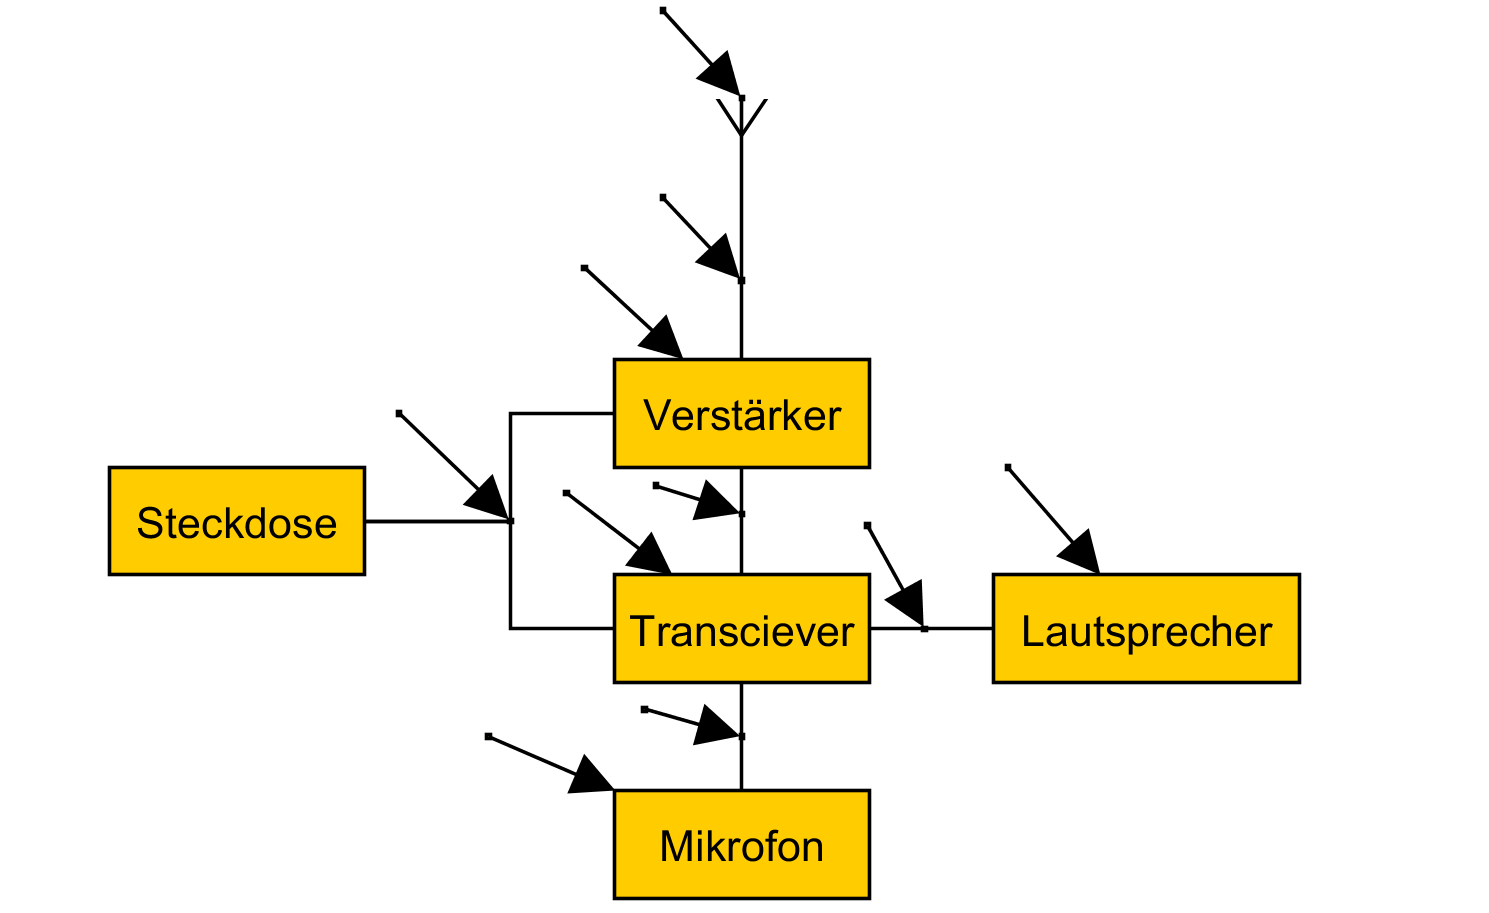
\includegraphics[width=1\textwidth,height=.75\textheight,keepaspectratio]{e18/Stoerungen.png}
    \attribcaption{Mögliche Einstrahlungspunkte}{DM7MD}{http://www.dk0tu.de/users/DM7MD/}{}
  \end{figure}
\end{frame}

\begin{frame}
  \frametitle{Was stört uns?}
  \begin{itemize}
    \item Intermodulationen (Übersteuern der Mischstufe durch mehrere, zu starke Signale)
    \item Diese erzeugen dann Phantomsignale
    \item Zustopfeffekte
  \end{itemize}
\end{frame}

\begin{frame}
  \frametitle{Prüfungsfrage}
  \begin{tabular}{l||p{.8\textwidth}}\hline
    \textbf{TK101} & \textbf{Wie äußert sich das Zustopfen bzw. Blockierung eines Empfängers?} \\ \hline\hline
    A & Durch das Auftreten von Pfeifstellen im gesamten Abstimmungsbereich. \\ \hline
    B \only<2>\checkmark & Durch den Rückgang der Empfindlichkeit und ggf. das Auftreten von Brodelgeräuschen. \\ \hline
    C & Durch eine zeitweilige Blockierung der Frequenzeinstellung. \\ \hline
    D & Durch Empfindlichkeitssteigerung. \\ \hline
  \end{tabular}
\end{frame}

\begin{frame}
  \frametitle{Prüfungsfrage}
  \begin{small}
    \begin{tabular}{l||p{.8\textwidth}}\hline
      \textbf{VG107} & \textbf{Der Empfang einer Amateurfunkaussendung wird auf der dem Amateurfunk ``primär'' zugewiesenen Frequenz 7,05 MHz durch den Schaltkontakt einer Heizungssteuerung aus der Nachbarschaft gestört. Was trifft für diesen Fall nach den Regelungen des EMVG bzw. AFuG zu?} \\ \hline
      A \only<2>\checkmark & Die Heizungssteuerung darf weiterbetrieben werden, wenn sie die für sie gültigen Grenzwerte aus den europäisch anerkannten Normen einhält. \\ \hline
      B & Die Heizungssteuerung ist außer Betrieb zu nehmen, da sie keine Aus\-sendung in einem Amateurfunkband machen darf. \\ \hline
      C & Die Heizungssteuerung muss umgehend außer Betrieb genommen werden, da sich die gestörte Frequenz in einem primär zugewiesenen Amateurfunkband befindet. \\ \hline
      D & Die Heizungssteuerung darf aus Gründen der Verhältnismäßigkeit unabhängig von der Einhaltung irgendwelcher Grenzwerte innerhalb der Heizperioden weiterbetrieben werden. \\ \hline
    \end{tabular}
  \end{small}
\end{frame}

\begin{frame}
  \frametitle{Vorbeugende Maßnahmen}
  \begin{itemize}
    \item Sendeanlage so weit weg von Empfangsantennen wie möglich aufbauen
    \item Eine Richtantenne mit geringem vertikalen Öffnungswinkel auf dem Dach ist ein guter Anfang
    \item Anpassen der Sendeleistung
  \end{itemize}
\end{frame}

\section{Personenschutz (EMVU)}

\begin{frame}
  \frametitle{Personenschutz (EMVU)}
  \begin{itemize}
    \item Es gilt zwei Bereiche zu beachten:
      \begin{itemize}
        \item Expositionsbereich 1 (Vom Funker kontrollierbarer Bereich) und
        \item Expositionsbereich 2 (Öffentlicher Bereich)
      \end{itemize}
    \item Es gibt festgelegte Grenzwerte und Formeln der BNetzA zur Berechnung des Sicherheitsabstandes
    \item Diverse Software zur Berechnung der Sicherheitsabstände
    \item Für eine ortsfeste Antenne ist (ab 10W EIRP) eine Selbsterklärung vor Betriebsaufnahme abzugeben
  \end{itemize}
\end{frame}

\begin{frame}
  \frametitle{Sicherheitsabstand}
  \begin{block}{Sicherheitsabstand}
    \begin{LARGE}
      $r = \frac{\sqrt{30 \cdot P_{EIRP}[W]}}{E[\frac{V}{m}]}$
    \end{LARGE}
  \end{block}
  \vspace{1em}

  \begin{center}
    \begin{tabular}{|c|c|}
      \hline
      \multicolumn{2}{|l|}{\textbf{Grenzwerte für Personenschutz}} \\ \hline
      \textbf{Frequenzbereich} & \textbf{Elektrische Feldstärke} \\ \hline
      0,1 - 1 MHz & $E = 87 \frac{V}{m}$ \\ \hline
      1 - 10 MHz & $E = \frac{87}{\sqrt{f}} \frac{V}{m}$ \\ \hline
      10 - 400 MHz & $E = 28 \frac{V}{m}$ \\ \hline
      400 - 2000 MHz & $E = 1,375 \cdot \sqrt{f} \frac{V}{m}$ \\ \hline
      über 2000 MHz & $E = 61 \frac{V}{m}$ \\ \hline
    \end{tabular}
  \end{center}
  Grenzwerte aus \href{https://www.gesetze-im-internet.de/bimschv\_26/anhang\_1.html}{\ExternalLink 26. BImSchV}
\end{frame}

\begin{frame}
  \begin{figure}
    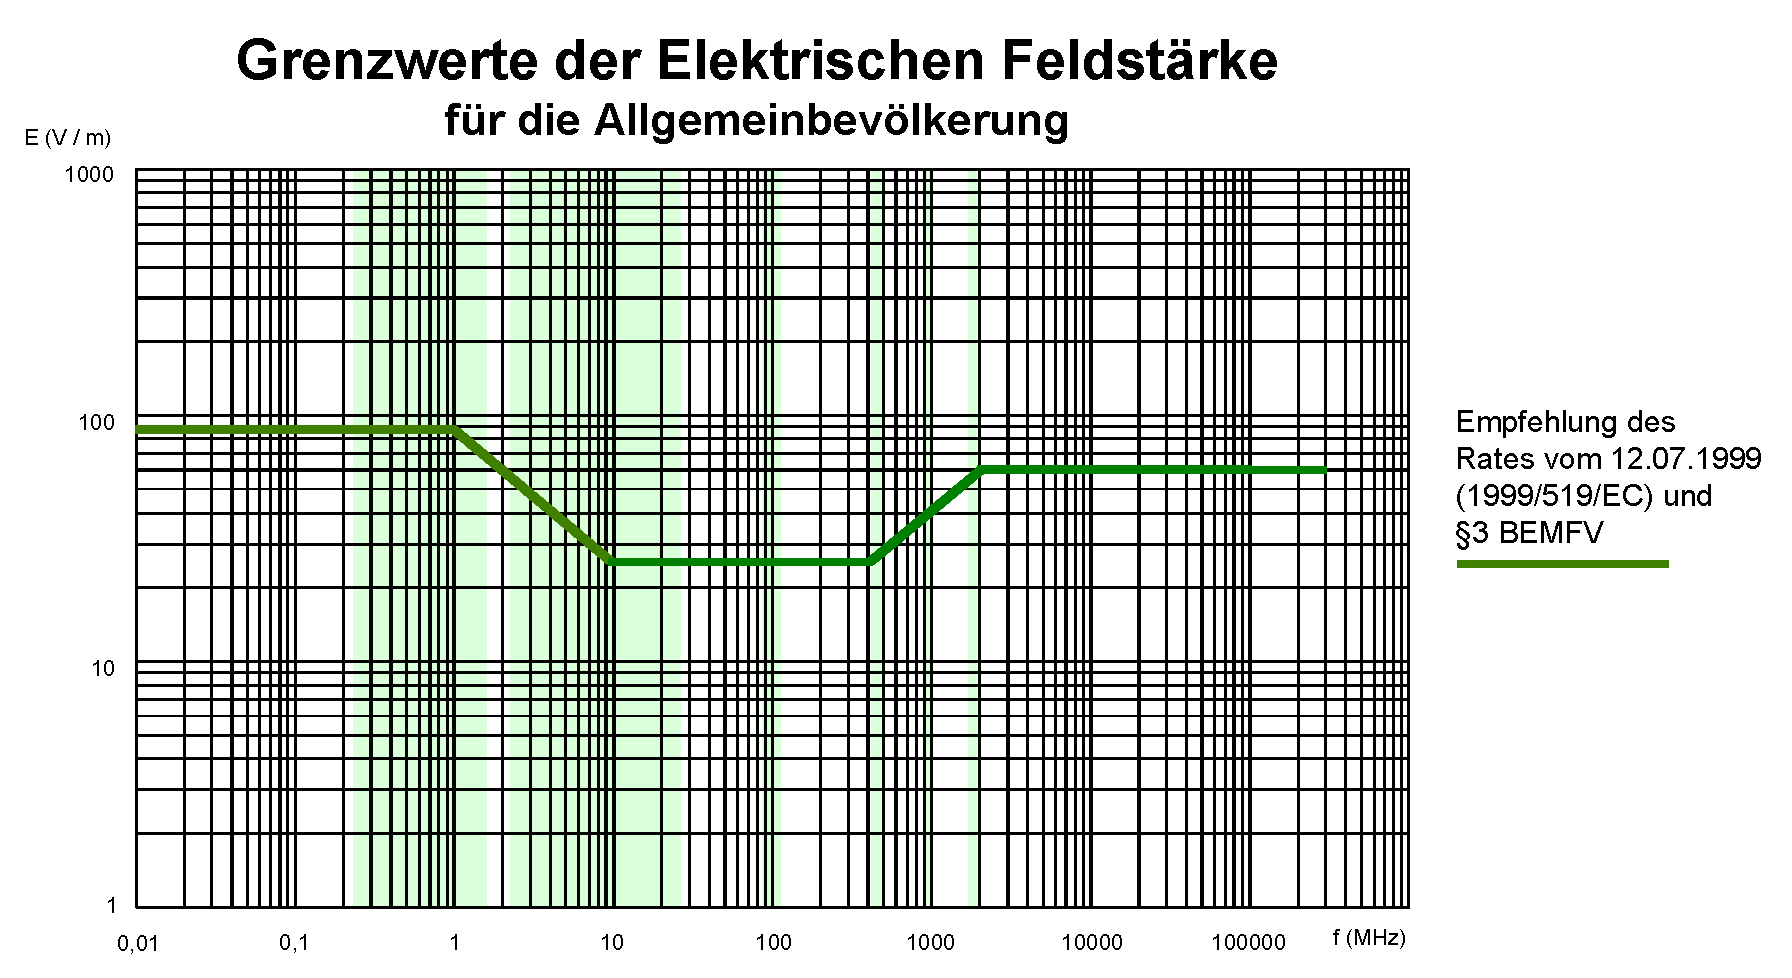
\includegraphics[width=\textwidth,height=.8\textheight,keepaspectratio]{e18/E_grenzkurve_gr.png}
    \attribcaption{Grenzwerte der Elektrischen Feldstärke}{Bundesnetzagentur}{http://emf3.bundesnetzagentur.de/Grenzwerte.html}{}
  \end{figure}
\end{frame}

\begin{frame}
  \frametitle{Leistungsgewinnfaktoren und Reduzierungsfaktoren}
  \begin{tabular}{|c|c|c|}
    \hline
    \multicolumn{2}{|l|}{\textbf{Leistungsgewinnfaktoren}} & \textbf{oder in dBi} \\ \hline
    Dipol & 1,64 & 2,15 dBi \\ \hline
    $\lambda / 4$ - Strahler & 3,28 & 5,15 dBi \\ \hline
  \end{tabular}
  \vspace{0.5cm}

  \begin{tabular}{|c|c|}
    \hline
    \textbf{Betriebsart} & \textbf{Reduzierungsfaktor} \\ \hline
    SSB & $1 : 6 = 0,167$ \\ \hline
    CW & $1 : 4 = 0,25$ \\ \hline
    FM (RTTY, SSTV) & 1 \\ \hline
  \end{tabular}\\[1.5em]
  Reduzierungsfaktoren sind Effektivwerte der maximalen Feldstärke gemittelt über ein 6-Minuten Intervall
\end{frame}

\begin{frame}
  \frametitle{Prüfungsfrage}
  \begin{tabular}{l||p{.8\textwidth}}\hline
    \textbf{TL209} & \textbf{Sie möchten den Personenschutz-Sicherheitsabstand für die Antenne Ihrer Amateurfunkstelle für das 10-m-Band und die Betriebsart RTTY berechnen. Der Grenzwert im Fall des Personenschutzes beträgt 28 V/m. Sie betreiben einen Dipol, der von einem Sender mit einer Leistung von 100W über ein Koaxialkabel gespeist wird. Die Kabeldämpfung sei vernachlässigbar. Wie groß muss der Sicherheitsabstand sein?} \\ \hline
    A & 5,01m \\ \hline
    B & 1,96m \\ \hline
    C \only<2>\checkmark & 2,50m \\ \hline
    D & 13,7m \\ \hline
  \end{tabular}
\end{frame}

\section{Sicherheit}

\begin{frame}
  \frametitle{Gesetze und Vorschriften, wohin man schaut}
  \begin{itemize}
    \item Selbstgebaute Geräte müssen den VDE-Bestimmungen entsprechen
    \item Für den Bau von Antennenanlagen gelten die Bauverordnungen des jeweiligen Landes
    \item Des Weiteren sind die Blitzschutzbestimmungen zu beachten
  \end{itemize}
\end{frame}

\subsection{elektrische Sicherheit}

\begin{frame}
  \frametitle{elektrische Sicherheit}
  \begin{itemize}
    \item Sicherheitsanforderungen
    \item Berührungsschutz
    \item Schutzkleinspannung \& Funktionskleinspannung
    \item Schutzisolierung
    \item Schutztrennung
    \item Schutz durch Abschalten
  \end{itemize}
\end{frame}

\begin{frame}
  \frametitle{Antennenerdung}
  Alle leitfähigen Teile der Antennenanlage müssen geerdet werden\\[1.5em]
  \begin{tabular}{|c|c|}
    \hline
    \textbf{Werkstoff} & \textbf{Abmessungen oder Art} \\ \hline
    Kupfer & $16 mm^2$, blank oder isoliert \\ \hline
    Aluminium & $25 mm^2$, isoliert, in Innenräumen auch blank \\ \hline
    Stahl & $50 mm^2$, verzinkt, z.B. Band $20mm \cdot 2,5mm$ \\ \hline
    \multicolumn{2}{|l|}{Volldraht oder mehrdrähtig, aber nicht feindrähtig} \\
    \multicolumn{2}{|l|}{Kennzeichnung der Erdleiter: grün-gelb} \\ \hline
  \end{tabular}
\end{frame}

\begin{frame}
  \frametitle{Blitzschutz}
  \begin{itemize}
    \item Antennenanlagen müssen gegen Blitze geschützt werden
    \item Der Mast muss auf dem kürzestem Weg mit einer fachlich korrekt installierten Gebäudeblitzschutzanlage verbunden werden
    \item Als Blitzschutzerder darf jeder ordnungsgemäß verlegter Fundamenterder verwendet werden
    \item Außenleiter von Koaxkabeln (Abschirmung) müssen über einen Potentialausgleichsleiter ordnungsgemäß mit Erde verbunden werden
  \end{itemize}
  \begin{center}
    \begin{figure}
      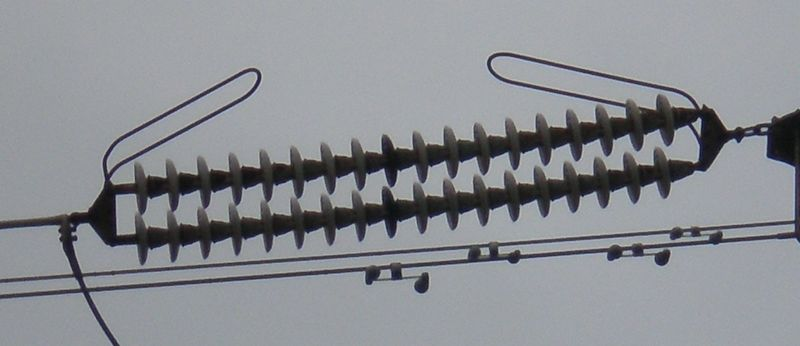
\includegraphics[width=.5\textwidth,height=.3\textheight,keepaspectratio]{e18/Funkenstrecke}
      \attribcaption{Funkenstrecke bei selbststrahlenden Sendemasten}{(Japanische Zeichen nicht darstellbar)}{http://de.wikipedia.org/wiki/Datei:Suspension_insulators_with_arcing_horns.jpg}{\ccby}
    \end{figure}
  \end{center}

\end{frame}

\begin{frame}
  \frametitle{Prüfungsfrage}
  \begin{tabular}{l||p{.8\textwidth}}\hline
    \textbf{TL301} & \textbf{Unter welchen Bedingungen darf das Standrohr einer Amateurfunkantenne auf einem Gebäude mit einer vorhandenen Blitzschutzanlage verbunden werden?} \\ \hline
    A \only<2>\checkmark & Wenn die vorhandene Blitzschutzanlage fachgerecht aufgebaut ist und das Standrohr mit ihr auf dem kürzesten Wege verbunden werden kann. \\ \hline
    B & Nach den geltenden Vorschriften muss das Standrohr der Amateurfunkantenne mit einer vorhandenen Gebäude-Blitzschutzanlage verbunden werden. \\ \hline
    C & Nach den geltenden Vorschriften muss immer eine eigene Blitzschutzanlage für eine Amateurfunkantenne aufgebaut werden. \\ \hline
    D & Die Bedingung ist ein ausreichend großer Querschnitt für die Verbindungsleitung zur Blitzschutzanlage. \\ \hline
  \end{tabular}
\end{frame}

\subsection{mechanische Sicherheit}

\begin{frame}
  \frametitle{mechanische Sicherheit}
  \begin{itemize}
    \item Sendeanlage muss mechanisch gesichert werden
    \item Windlast ist zu beachten
  \end{itemize}
  \begin{block}{Kraft auf eine Antennenanlage}
    \Large{$F_{A} = p \cdot A$}
  \end{block}
  \begin{itemize}
    \item Sendeanlagen dürfen im KFZ installiert werden
    \item Dafür immer Herstellerangaben beachten
    \item Um Störungen zu vermeiden, Antenne und Antennenkabel möglichst weit weg von      Fahrzeugelektronik installieren
  \end{itemize}
\end{frame}

\renewcommand{\refname}{Referenzen}

\hypertarget{refs}{}
\textcolor{white}{} \\ %\vspace{} geht nicht
\Large Referenzen/Links
\footnotesize

\begin{thebibliography}{}
  \bibitem{bv14}  Moltrecht B/V 14: \\
    \url{https://www.darc.de/der-club/referate/ajw/lehrgang-bv/bv14/}
  \bibitem{e18}   Moltrecht E 18: \\
    \url{https://www.darc.de/der-club/referate/ajw/lehrgang-te/e18/}
  \bibitem{wp}    Wikipedia DE: \\
    \url{http://de.wikipedia.org/wiki/Blitzschutz}\\
    \url{http://de.wikipedia.org/wiki/Funkenstrecke}\\
\end{thebibliography}

% Hier könnte noch eine Kontaktfolie stehen

\end{document}

